\documentclass[11pt]{ctexbook}

\usepackage{amsmath}
\usepackage{amssymb}
\usepackage{bm}

\usepackage{algorithm}
\usepackage{algorithmic}

\usepackage{hyperref}
\usepackage{graphicx}

\title{\textbf{PRML读书笔记} }
\author{C. Lu}


\begin{document}

\maketitle
\tableofcontents

\chapter{绪论}
\section{概率论}
概率论的两条基本法则:
\begin{equation} 
	\mathrm{\textbf{sum rule}} \ \ p(X) = \sum_Y p(X, Y)
\end{equation}
\begin{equation} 
	\mathrm{\textbf{product rule}} \ \ p(X, Y) = p(Y\ |\ X)p(X)
\end{equation}
其中$p(X, Y)$是联合概率分布,表示是\ “$X$且$Y$的概率”;$P(Y\ |\ X)$是条件概率,表示为“给定$X$的条件下, $Y$发生的概率”。

根据对称性\ $p(X, Y) = p(Y, X)$, 可以推导出:
\begin{equation}
	\label{eq:bayes}
	p(Y\ |\ X) = \frac{p(X\ |\ Y)p(Y)}{p(X)}
\end{equation}
公式\ref{eq:bayes}被称为\emph{贝叶斯定理}(Bayes' theorem)。使用加和法则,贝叶斯定理中的分母可以用出现在分子中的项表示:
\begin{equation}
	p(X) = \sum_Y p(X\ |\ Y)p(Y)
\end{equation}
\subsection{概率密度}
对于连续型随机变量$x$ 位于区间$ (a, b)$上的概率由下式给出:
\begin{equation}
	p(x\in(a, b)) = \int_{a}^{b}p(x)\ \mathrm{d}x
\end{equation}
由于概率是非负的,并且$x$的值一定位于实数轴的某个位置,因此概率密度一定满足以下两个条件:
\begin{equation}
	p(x) \geqslant 0
\end{equation}
\begin{equation}
	\int_{-\infty}^{+\infty}p(x)\ \mathrm{d}x= 1
\end{equation}

我们考虑一个随机变量的转换$x = g(y)$,$p_x(x)$与$p_y(y)$分别代表了$x$与$y$的概率密度函数,对于很小的$\delta_x$,落在区间$(x,\ x+\delta_x)$内的观测值会被变换到$(y,\ y+\delta_y)$中。其中$p_x(x)\delta_x \simeq p_y(y)\delta_y$,因此
\begin{equation}
	p_y(y) = p_x(x)\left|\frac{\mathrm{d}x}{\mathrm{d}y}\right| = p_x(g(y))\left|g'(y)\right|
\end{equation}
这个性质说明了概率密度最大值的位置,取决于变量的选择。

位于区间$(-\infty,\ z)$的$x$的概率密度由累积分布函数(c.d.f)给出。定义为:
\begin{equation}
	P(z) = \int_{-\infty}^{z}p(x)\ \mathrm{d}x
\end{equation}
满足$P'(x) = p(x)$。

如果有多个连续变量$x_1, x_2, \ldots, x_D$,整体记作向量$\bm x$,那么我们可以定义联合概率密度$p(\bm x) = p(x_1, x_2, \ldots, x_D)$,使得$\bm x$落在包含点$\bm x$的无穷小体积$\delta_{\bm x}$的概率由$p(\bm x) \delta_{\bm x}$给出。多便利那个概率密度必须满足
\begin{equation}
	p(\bm x) \geqslant 0
\end{equation}
\begin{equation}
	\int p(\bm x)\ \mathrm{d}\bm x = 1
\end{equation}
其中积分必须在整个$\bm x$的空间上进行。

概率密度的加和规则、乘积规则以及贝叶斯规则同样可以应用到连续变量的概率密度函数上,也可以应用到离散变量和连续变量的混合的情形。若$x$, $y$是两个连续变量,那么加和规则和乘积规则为
\begin{equation}
	p(x) = \int p(x, y)\ \mathrm{d}y
\end{equation}
\begin{equation}
	p(x, y) = p(y\ |\ x)p(x)
\end{equation}
形式化证明连续变量的加和规则和乘积规则需要用到\emph{测度论}的数学分支。

\subsection{期望和方差}
\section{信息论}

\chapter{概率分布}
\section{二元变量}
首先考虑一个二元变量$x \in \{0, 1\}$,其中$x=1$的概率记作参数$\mu$,
\begin{equation}
	p(x=1\ |\ \mu) = \mu
\end{equation}
其中$0 \leq \mu \leq 1$。显然,$p(x=0\ |\ \mu) = 1-\mu$。$x$的概率分布因此可以写成
\begin{equation}
	\mathrm{Bern}(x \ |\ \mu) = \mu^x(1-u)^{1-x}
\end{equation}
这叫做\emph{伯努利分布}。分布的均值和方差
\begin{equation}
	\mathbb E[x] = \mu
\end{equation}
\begin{equation}
	\mathrm{Var}[x] = \mu(1-\mu)
\end{equation}
现在假设有一个观测数据集$\mathcal D = \{x_1, \ldots, x_N\}$,且每次观测数据都是独立地从$p(x\ |\ \mu)$中抽取的,因此可以构造关于$\mu$的似然函数
\begin{equation}
	p(\mathcal D \ |\ \mu) = \prod_{n=1}^{N}p(x_n\ |\ \mu) = \prod_{n=1}^{N}\mu^{x_n}(1-\mu)^{1-x_n}
\end{equation}
以频率学家的观点来看,可以通过最大化似然函数来估计$\mu$的值,或者,等价的,最小化交叉熵。在伯努利分布的形式下,对数似然函数为
\begin{equation}
	\log p(\mathcal D \ |\ \mu) = \sum_{n=1}^{N}\log p(x_n\ |\ \mu) = \sum_{n=1}^{N}\left\{ x_n\log \mu + (1-x_n)\log(1-\mu) \right\}
\end{equation}
如果令$\log p(\mathcal{D}\ |\ \mu)$关于$\mu$的导数等于零,就得到了最大似然的估计值
\begin{equation}
	\label{eq:bern_ml}
	\mu_{\mathrm{ML}} = \frac{1}{N}\sum_{n=1}^{N}x_n
\end{equation}
这样称为样本均值。如果我们把数据集里$x=1$的观测数量记作$m$,那么可以把公式\ref{eq:bern_ml}写成下面的形式
\begin{equation}
	\mu_{\mathrm{ML}} = \frac{m}{N}
\end{equation}

\section{多项式变量}
\section{高斯分布}
\section{指数族分布}

\chapter{线性回归模型}
\section{线性函数模型}
\subsection{最大似然与最小平方误差}
\subsection{最小平方误差的几何解释}
\subsection{正则化的最小平方误差}
\section{偏差-方差分解}
\section{贝叶斯线性回归}
\subsection{参数分布}
\subsection{预测分布}

\chapter{线性分类模型}

\chapter{核方法}

\chapter{稀疏核机}
\section{最大边缘分类器}

\chapter{图模型}
\section{贝叶斯网络}

\chapter{混合模型和EM}
\section{K-means 算法}
假设有一个数据集$\{ \bm x_1, \bm x_2, \ldots, \bm x_N\}$,它由$D$维欧几里得空间中的随机变量$\bm x$的$N$次观测组成。我们的目的是要将数据划分成$K$个类别,假设$K$是给定的一个数。

引入一组$D$维向量$\bm \mu_k$,其中$k=1, 2, \ldots, K$,且$\bm \mu_k$是第$k$个聚类关联的一个代表,可以认为$\bm \mu_k$是第$k$个聚类的中心。算法的目的是要找到每个数据点分别属于的类,以及一组向量$\{\bm \mu_k\}$,使得每个数据点和它最近的向量$\bm \mu_k$之间的距离的平方和最小。

现在,对于每个数据点$\bm x_n$,引入一组对应的二值指示变量$r_{nk} \in \{0, 1\}$,其中 $k = 1, 2, \ldots, K$,表示每个数据点$\bm x_n$属于$K$个聚类中的。如果数据点$\bm x_n$属于第$k$个聚类,那么$r_{nk}=1$,且对于$j \neq k$, 有$r_{nj} = 0$。定义目标函数,形式为:
\begin{equation}
	\label{eq:kmeas-cost}
	J = \sum_{n=1}^{N}\sum_{k=1}^{k}r_{nk}\| \bm x_n - \bm \mu_k \|^2
\end{equation}
它表示每个数据点与被分配的向量$\bm \mu_k$之间的距离的平方和。我们的目标是要找到$\{r_{nk}\}$与$\bm \mu_{nk}$的值,使得$J$达到最小值。

可以使用迭代的方法来达到目标。每次迭代分为两个步骤,分别对应$r_{nk}$的最优化和$\bm \mu_k$的最优化。 首先,为$\bm \mu_k$选择一些初始值。然后,在第一阶段,关于$r_{nk}$最小化$J$,保持$\bm \mu_k$固定。第二阶段,关于$\bm \mu_k$最小化$J$,保持$r_{nk}$固定。不断重复这个二阶段优化直到收敛。

首先考虑确定$r_{nk}$。公式\ref{eq:kmeas-cost}关于$r_{nk}$是线性的,且与不同的$n$相关的项是独立的,可以对每个$n$分别进行优化。只要$k$的值使$\|\bm x_n-\bm \mu_k\|^2$的值最小,就令$r_{nk}=1$,换句话说,可以简单的将数据点的聚类设置为最近的聚类中心。形式化的表述为
\begin{equation}
	r_{nk} = \left\{\begin{array}{ll}
		1, & \text{如果} k = \arg\min_{j} \| \bm x_n - \bm \mu_j\|^2 \\
		0, & \text{其他情况}
	\end{array}\right.
\end{equation}

现在考虑$r_{nk}$固定时,关于$\bm \mu_K$的最优化。目标函数$J$是一个二次函数,令它关于$\bm \mu_k$的导数等于$0$,即可达到最小值,即
\begin{equation}
	2\sum_{n=1}^{N}r_{nk}(\bm x_n - \bm \mu_k) = 0
\end{equation}
解出$\bm \mu_k$的值,结果为
\begin{equation}
	\label{eq:u_k}
	\bm \mu_k = \frac{\sum_n r_{nk}\bm x_n}{\sum_n r_{nk}}
\end{equation}
\ref{eq:u_k}中的分母等于聚类$k$中数据点的数量,因此这个结果的意义是:$\mu_k$为聚类$k$中所有数据点的均值。因此,此算法被称为K-means算法。

重新为数据点分配聚类的步骤以及重新计算聚类均值的步骤重复进行,直到聚类的分配不再改变。每个阶段都减小了目标函数$J$,因此算法的收敛性得到保证。但是,\emph{算法可能收敛到$J$的一个局部最小值而非全局最小}。

\section{混合高斯}
高斯混合模型的概率分布可以写成多个高斯分布的线形叠加,即
\begin{equation}
	p(\bm x) = \sum_{k=1}^{K}\pi_k\mathcal N(\bm x\ | \ \bm \mu_k, \bm \Sigma_k)
\end{equation}
引入一个$K$维的二值随机变量$\bm z$, 采用“1-of-K”编码,其中一个特定的元素$z_k$等于$1$,其余所有的元素都等于$0$。 于是$z_k$的值满足$z_k \in \{0, 1\}$且$\sum_k z_k = 1$,并且我们看到根据哪个元素非零,向量$\bm z$有$K$个可能的状态。$\bm z$的边缘概率分布可以根据混合系数$\pi_k$进行赋值,即
\begin{equation}
	p(z_k=1) = \pi_k
\end{equation}
其中参数$\{\pi_k\}$必须满足
\begin{equation}
	0 \leqslant \pi_k \leqslant 1
\end{equation}
以及
\begin{equation}
	\sum_{k=1}^{K} \pi_k = 1
\end{equation}
由于$\bm z$使用了“1-of-K”编码,也可以将这个概率分布写成
\begin{equation}
	p(\bm z) = \prod_{k=1}^{k}\pi_k^{z_k}
\end{equation}
对于$\bm z$给定的一个值, $\bm x$的条件概率分布是一个高斯分布
\begin{equation}
	p(\bm x\ |\  z_k= 1) = \mathcal N (\bm x\ |\ \bm \mu_k, \bm \Sigma_k )
\end{equation}
类似的也可以写成
\begin{equation}
	p(\bm x \ | \ \bm z) = \prod_{k=1}^{K} \mathcal N (\bm x \ |\ \bm \mu_k, \bm \Sigma_k ) ^ {z_k}
\end{equation}

$\bm x $的边缘概率分布可以通过将联合概率分布对所有可能的$\bm z$求和的方式得到,即
\begin{equation}
	p(\bm x) = \sum_z p(\bm z)p(\bm x \ |\ \bm z) = \sum_{k=1}^{K}\pi_k \mathcal N(\bm x \ |\ \bm \mu_k, \bm \Sigma_k)
\end{equation}
于是我们找到了一个将隐变量$\bm z$显示写出的一个高斯混合分布一个等价公式。对联合概率分布$p(\bm x, \bm z)$而不是对$p(\bm x)$进行操作,会产生计算上极大的简化。

另一个有重要作用的量是给定$\bm x$的情况下,$\bm z$的后验概率$p(\bm z\ |\ \bm x)$。用$\mathcal \gamma(z_k)$表示$p(z_k=1\ |\ \bm x)$,其值可由贝叶斯定理给出
\begin{align}
	\gamma(z_k) = p(z_k=1\ |\ \bm x) &= \frac{p(z_k=1)p(\bm x\ |\ z_k=1)}{\sum_{j=1}^{K}p(z_j=1)p(\bm x\ |\ z_j=1)} \\
									 &= \frac{\pi_k p(\bm x\ |\ z_k=1)}{\sum_{j=1}^{K}\pi_j p(\bm x\ |\ z_j=1)} 
\end{align}
可以将$\pi_k$看成是$z_k=1$的先验概率,将$\gamma(z_k)$看成是观测到$\bm x$之后,对应的后验概率。

假设我们有观测数据集$\{\bm x_1, \bm x_2, \ldots, \bm x_N\}$,我们希望使用混合高斯来对数据建模。可以将这个数据集标示为$N\times D$的矩阵$\bm X$,其中第$n$行为$\bm x_n^\top$。类似的,对应的隐变量被表示为一个$N\times K$的矩阵$\bm Z$,它的行为$\bm z_n^\top$,可以使用图\ref{fig:em-model} 所示的图模型来表示独立同分布数据集的高斯混合模型。$\bm X$的对数似然函数为
\begin{equation}
	\label{eq:6-15}
	\log p(\bm X\ |\ \bm \pi, \bm \mu, \bm \Sigma)=\sum_{n=1}^{N}\log\left\{ \sum_{k=1}^{K}\pi_k\mathcal N(\bm x_n\ |\ \bm \mu_k, \Sigma_k) \right\}
\end{equation}
最大化高斯混合模型的对数似然函数式\ref{eq:6-15}比单一的高斯分布的情形更加复杂。因为对$k$的求和出现在了对数内部;\emph{如果令导数等于零,不会得到一个解析解}。
使用基于梯度的优化方法可以得到解,但现在考虑另一种可行方法,称为\emph{EM算法}。

\section{EM 算法}
期望最大化算法,也叫EM算法,是寻找潜在变量的概率模型的最大似然解的一种通用方法。考虑一个概率模型,其中所有的观测变量记作$\bm X$,所有隐含变量记作$\bm Z$。联合概率分布$p(\bm X, \bm Z\ |\ \bm \theta)$由一组参数$\bm \theta $控制,目标是最大化似然函数
\begin{equation}
	p(\bm X\ |\ \bm \theta) = \sum_{\bm Z}p(\bm X, \bm Z | \bm \theta)
\end{equation}
这里,假设$\bm Z$是离散的。
\begin{figure}
	\centering
	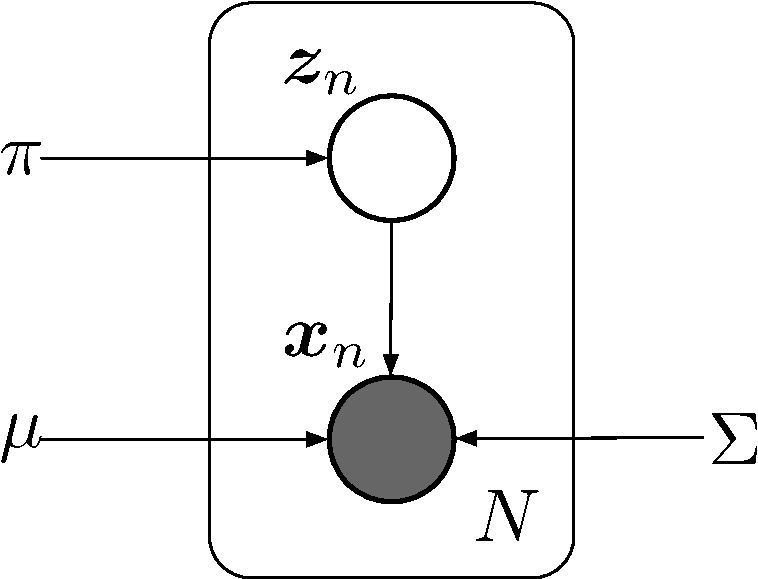
\includegraphics[width=6cm]{EM-model}
	\caption{一组N个独立同分布数据点$\{\bm x_n\}$的高斯混合模型的图表示,对应的潜在变量为$\{\bm z_n\}$,其中$n=1,2,\ldots, N$。}
	\label{fig:em-model}
\end{figure}
直接优化$p(\bm X\ |\ \bm\theta)$比较困难,但是最优化完整数据似然函数$p(\bm X, \bm Z\ |\ \bm \theta)$就容易得很多。接下来,引入一个定义在隐变量$\bm Z$上的分布$p(\bm Z)$。对任意$p(\bm Z)$,如下分解成立
\begin{equation}
	\log p(\bm X\ |\ \bm\theta) = \mathcal L(q, \bm \theta) + \mathrm{KL}(q\ \|\ p)
\end{equation}
其中
\begin{equation}
	\mathcal L(q, \bm\theta) = \sum_{\bm Z}q(\bm Z)\log\left\{ \frac{p(\bm X,\bm Z\ |\ \bm \theta)}{q(\bm Z)}\right\}
\end{equation}
\begin{equation}
	\mathrm{KL}(p\ \|\ q) = -\sum_{\bm Z}q(\bm Z)\log\left\{\frac{p(\bm Z\ |\ \bm X, \bm\theta)}{q(\bm Z)}\right\}
\end{equation}
$\mathcal L(q, \bm\theta)$是概率分布$q(\bm Z)$的一个\emph{范函},并且是一个参数$\bm\theta$的函数。因为$\mathrm{KL}(p\ \|\ q) \geqslant 0$,当且仅当$q(\bm Z) = p(\bm Z\ |\ \bm X, \bm\theta)$时取得等号。因此,$\mathcal L(q, \bm\theta) \leqslant \log p(\bm X\ |\ \bm\theta)$,即$\mathcal L(q, \bm\theta)$是$\log p(\bm X\ |\ \bm\theta)$是的一个下界。

EM算法是一个两阶段迭代优化算法。

假设当前的参数$\bm\theta^{\mathrm{old}}$,在\emph{E步骤}中,下界$\mathcal L(q, \bm\theta^{\mathrm{old}})$关于$q(\bm Z)$最大化,而$\bm\theta^{old}$保持固定。当KL散度为零时,即得到了最大化的解。换句话说,最大值出现在$q(\bm Z)$与后验概率分布$p(\bm Z\ |\ \bm X, \bm\theta)$相等时,KL散度等于零,此时,下界等于最大似然函数。

在接下来的\emph{M步骤}中,分布$q(\bm Z)$保持固定,下界$\mathcal L(q, \bm\theta)$关于$\bm\theta$最大化,得到了某个新的值$\bm\theta^{\mathrm{new}}$,这会使得下界$\mathcal L$增大。同时也会使得对数似然增大,因为概率分布$q$由旧的参数值确定,并且在\emph{M步骤}保持固定,因此不会等于新的后验分布$p(\bm Z\ |\ \bm X,\bm\theta^{\mathrm{new}})$,从而KL散度非零;而且对数似然的增加量大于下界$\mathcal L(q, \bm\theta)$的增加量。在\emph{E步骤}之后,下界的形式为
\begin{align*}
	\mathcal L(q, \bm\theta) &= \sum_{\bm Z}p(\bm Z\ |\ \bm X, \bm\theta^{\mathrm{old}})\log p(\bm X, \bm Z\ |\ \bm\theta)\\
	& \ \ \ \ - \sum_{\bm Z}p(\bm Z\ |\ \bm X,\bm\theta^{\mathrm{old}})\log p(\bm Z\ |\ \bm X, \bm\theta^{\mathrm{old}}) \\
	&= \mathcal Q(\bm\theta, \bm\theta^{\mathrm{old}}) + \text{常数}
\end{align*}
其中常数是$q$的熵,与$\bm \theta$无关。从而,在\emph{M步骤}中,最大化的量是\emph{完整数据对数似然函数的期望}。完整的EM如算法\ref{algo:em}所示。
\begin{algorithm}
\caption{用于含有隐变量最大似然函数参数估计的EM算法}
\label{algo:em}
\begin{algorithmic}[1]
\STATE 选择参数的初始值$\bm\theta^{(t)}, t = 0$
\REPEAT
\STATE \textbf{E步骤}:\ \ 计算$p(\bm Z\ |\ \bm X, \bm\theta^{(t)})$
\STATE \textbf{M步骤}:\ \ 计算$\bm\theta^{(t+1)}$,由下式给出
\begin{equation*}
	\bm \theta^{(t+1)} = \arg\max_{\bm \theta}\mathcal Q (\bm\theta, \bm\theta^{(t)})
\end{equation*}
其中
\begin{equation*}
	\mathcal Q (\bm\theta, \bm\theta^{(t)}) = \sum_{\bm Z}p(\bm Z\ |\ \bm X, \bm \theta^{(t)}) \log p(\bm X, \bm Z\ |\ \bm\theta)
\end{equation*}
\UNTIL{对数似然函数收敛或者参数值收敛}
\end{algorithmic}
\end{algorithm}

\section{EM算法实例}
\subsection{用于混合高斯模型的EM}

\subsection{伯努利分布的混合}
\chapter{近似推断}

\chapter{采样方法}
\section{基本算法}
\subsection{概率分布采样}
\subsection{拒绝采样}
\subsection{重要性采样}
\section{马尔可夫链蒙特卡罗方法}
\subsection{马尔可夫链}
\subsection{Metropolis-Hastings算法}
\section{吉布斯采样}

\chapter{连续潜在变量}
\section{主成分分析}
主成分分析,或者称为PCA,是一种广泛使用的技术,应用的领域包括维度降低、有损数据压缩、特征抽取、数据可视化。有两种经常使用的PCA的定义:
\begin{itemize}
	\item PCA被定义为数据在被称为\emph{主子空间}的低维线性空间上的投影,使得投影数据的方差最大化
	\item 也可以被定义为使得平均投影代价最小的线性投影,平均投影代价是指数据点和它们的投影之间的平均平方距离
\end{itemize}
\subsection{最大方差形式}
考虑一组观测数据集${\bm x_n}$,其中$n=1,\ldots,N$,$\bm x_n$是一个$D$维欧几里得空间中的变量。考虑将数据投影到维度是$M<D$的空间中。

首先,考虑在一维空间$(M=1)$上的投影。可以使用$D$维向量$\bm u_1$定义投影方法。为了计算方便和不失一般性,假定选择一个单位向量,而且$\bm u_1^{\top}\bm u_1 = 1$,这样每个数据点$\bm x_n$被投影到一个标量值$\bm u_1^{\top}\bm x_n$上。被投影数据的均值是$\bm u_1^{\top}\overline{\bm x}$,其中$
\overline{\bm x}$是样本集合的均值,形式为
\begin{equation}
	\overline{\bm x} = \frac{1}{N}\sum_{n=1}^{N}\bm x_n
\end{equation}
投影数据的方差为
\begin{equation}
	\frac{1}{N}\sum_{n=1}^{N}\{\bm u_1^{\top}\bm x_n - \bm u_1^{\top}\overline{\bm x}\}^2 = \bm u_1^\top\bm S\bm u_1
\end{equation}
其中$\bm S$是协方差矩阵,定义为
\begin{equation}
	\bm S = \frac{1}{N}\sum_{n=1}^{N}(\bm x_n - \overline{\bm x})(\bm x_n - \overline{\bm x})^\top
\end{equation}
现在关于$\bm u_1$最大化投影方差$\bm u_1^\top\bm S\bm u_1$,包含约束条件$\|\bm u_1\| = 1$。可以采用拉格朗日乘数法,转化为如下的无约束优化问题
\begin{equation}
	\bm u_1^\top \bm S\bm u_1 + \lambda_1(1-\bm u_1^\top\bm u_1)
\end{equation}
通过令其关于$\bm u_1$导数等于零,可以看到驻点满足
\begin{equation}
	\bm S\bm u_1 = \lambda_1\bm u_1
\end{equation}
这表明$\bm u_1$一定是$\bm S$的一个特征向量。如果左乘$\bm u_1^\top$,可以看到方差为
\begin{equation}
	\bm u_1^\top \bm S\bm u_1 = \lambda_1
\end{equation}
因此当我们将$\bm u_1$设置为与具有最大特征值$\lambda_1$的特征向量时,方差会达到最大值。这个特征向量被称为\emph{第一主成分}。

可以使用类似的方法定义额外的主成分,方法是:在与所有已经考虑过的方向正交的方向中,选择使得投影数据方差最大化的方向。例如,我们考虑$M$维投影空间的情况,那么最大化投影数据方差的方向由协方差矩阵$\bm S$的$M$个特征向量$\bm u_1, \bm u_2, \ldots, \bm u_M$定义,对应的$M$个特征值是$\lambda_1, \lambda_2, \ldots, \lambda_M$。

总结一下,主成分分析涉及计算数据集的均值$\overline{\bm x}$和协方差矩阵$\bm S$,然后寻找与$\bm S$对应的$M$个最大特征值的特征向量。寻找一个$D\times D$矩阵的完整的特征向量分解的代价为$\bm O(D^3)$。若只将数据投影到前$M$个主成分中,那么只需要寻找前$M$个特征向量和特征值,这可以使用更高效的算法,时间复杂度为$\bm O(MD^2)$,或者也可以使用EM算法。
\subsection{最小误差形式}
PCA的另一种形式,基于最小投影误差。先引入一个完备的单位正交集合$\{\bm u_i\}$,其中$i=1, \ldots, D$,且满足
\begin{equation}
	\bm u_i^\top \bm u_j = \delta_{ij}
\end{equation}
由于是完备的,因此每个数据点可以唯一的表示为一个线性组合,即
\begin{equation}
	\bm x_n = \sum_{i=1}^{D}\alpha_{ni}\bm u_i
\end{equation}
其中,系数$\alpha_{ni}$对于不同的数据点来说是不同的。这相当于将坐标系旋转到了一个由$\{\bm u_i\}$表示的新坐标系。我们有$\alpha_{nj} = \bm x_n^\top \bm u_j$,不失一般性,我们有
\begin{equation}
	\label{eq:pca-9-9}
	\bm x_n = \sum_{i=1}^{D}(\bm x_n^\top \bm u_i)\bm u_i
\end{equation}
我们的目标是限定数量$M<D$个变量的一种表示来近似数据点,这对应于在低维子空间的一个投影。因此,我们可以用下式来近似每个数据点$\bm x_n$
\begin{equation}
	\label{eq:pca-x_n}
	\tilde{\bm x}_n = \sum_{i=1}^{M}z_{ni}\bm u_i + \sum_{i=M+1}^{D}b_i\bm u_i
\end{equation}
其中$\{z_{nj}\}$依赖于特定的数据点,而$\{b_i\}$是常数,对于所有的数据点都相同。可以选择$\{\bm u_i\}$,$\{z_{ni}\}$,$\{b_i\}$,从而最小化由维度降低带来的失真。失真的度量,可以使用原始数据点与它近似点$\title{\bm x}_n$之间的平方距离。因此目标函数是
\begin{equation}
	J = \frac{1}{N}\sum_{n=1}^{N}\|\bm x_n - \tilde{\bm x}_n \|^2
\end{equation}
考虑关于$\{z_{ni}\}$的最小化。代入$\tilde{\bm x}_n$的表达式,然后令它关于$z_{nj}$的导数等于零,有
\begin{equation}
	z_{nj} = \bm x_n^\top\bm u_j
\end{equation}
其中$j=1, \ldots, M$;类似地,令$J$关于$b_i$的导数等于零,我们有
\begin{equation}
	b_j = \overline{\bm x}^\top\bm u_j
\end{equation}
其中,$j=M+1, \ldots, D$。将$z_{nj}$与$b_j$代入到式\ref{eq:pca-x_n}中,使用式\ref{eq:pca-9-9}中$\bm x_n$的展开式,可以得到
\begin{equation}
	\bm x_n - \tilde{\bm x}_n= \sum_{i=M+1}^{D}\left\{ (\bm x_n - \overline{\bm x})^\top \bm u_i\right\} \bm u_i
\end{equation}
然后就得到了失真度量$J$的表达式,它是一个纯粹的关于$\{\bm u_i\}$的函数,形式为
\begin{equation}
	J = \frac{1}{N}\sum_{n=1}^{N}\sum_{i=M+1}^{D}(\bm x_n^\top\bm u_i - \overline{\bm x}^\top\bm u_i)^2  = \sum_{i=M+1}^{D}\bm u_i^\top\bm S\bm u_i
\end{equation}

\subsection{高维数据的PCA}
在PCA的一些应用中,会出现数据维度远大于数据样本的个数。例如将PCA应用到由几百张图片构成的数据集合,此时,每个图片的维度为几百万维,远大于样本个数。若数据维度为$D$,样本个数为$N$,$(N << D)$,$N$个数据点定义了一个最多为$N-1$维的子空间,运行PCA会发现至少$N-D+1$个特征值为零;另外,寻找$D\times D$矩阵的特征向量算法的计算复杂度为$\bm O(D^3)$,对于高维度的数据来说,在计算上也不可行。

可以使用下面的方法解决这个问题。$\bm X$定义为$(D\times D)$维中心数据矩阵,它的第$n$行为$(\bm x_n - \overline{\bm x})^\top$。这样,数据的协方差矩阵可以写作$\bm S = \frac{1}{N}\bm X^\top \bm X$,对应的特征向量方程变成了
\begin{equation}
	\frac{1}{N}\bm X^\top \bm X\bm u_i = \lambda_i\bm u_i
\end{equation}
将两侧左乘一个$\bm X$,可得
\begin{equation}
	\frac{1}{N}\bm X \bm X^\top(\bm X\bm u_i) = \lambda_i(\bm X\bm u_i)
\end{equation}
若定义$\bm v_i = \bm X\bm u_i$,就有
\begin{equation}
\label{eq:h_pca}
	\frac{1}{N}\bm X\bm X^\top\bm v_i = \lambda_i\bm v_i
\end{equation}
它是$N\times N$矩阵$\frac{1}{N}\bm X\bm X^\top$的一个特征向量方程,且这个矩阵与原始的协方差矩阵有相同的$N-1$个特征值,原始协方差矩阵本身还有额外$D-N+1$个值为零的特征值。我们可以在低维空间中解决这个问题,计算代价是$\bm O(N^3)$而不是$\bm O(D^3)$。

为了得到原始协方差矩阵的特征向量,可以将公示\ref{eq:h_pca}两侧左乘$\bm X^\top$,得
\begin{equation}
	(\frac{1}{N}\bm X^\top\bm X)(\bm X^\top\bm v_i) = \lambda_i(\bm X^\top\bm v_i)
\end{equation}
从中,我们可以看到,$(\bm X^\top \bm v_i)$是原始数据协方差矩阵的一个特征向量,对应的特征值是$\lambda_i$。但是,这个特征向量的长度不一定为$1$,即$\bm u_i \propto \bm X^\top \bm v_i$。将此向量归一化,就可以得到$\bm u_i$,且$\|\bm u_i\|=1$。假设$\bm v_i$是单位向量,可以通过以下方式归一化
\begin{equation}
	\label{eq:u_i}
	\bm u_i = \frac{1}{(N\lambda_i)^\frac{1}{2}}\bm X^\top\bm v_i
\end{equation}

总结一下,使用这种方法,首先计算$\bm X \bm X^\top$,然后找到它的特征向量和特征值,之后使用公式\ref{eq:u_i}计算原始数据协方差矩阵的特征向量。
\section{概率PCA}
\section{核PCA}
\section{非线形隐变量模型}
\subsection{独立成分分析}
\subsection{自编码器}
\section{非线性流行建模}

\chapter{组合模型}

\end{document}
